\chapter{Background}

\section{Cryptographic Hash Functions}

A cryptographic hash function is a hash function that is suitable for use
in cryptography. It is a mathematical algorithm that maps data of arbitrary
size (often called the ``message'') to a bit string of a fixed size (the ``hash
value'', ``hash'', or ``message digest'') and is a one-way function, that is, a
function which is practically infeasible to invert. Ideally, the only way to
find a message that produces a given hash is to attempt a brute-force search of
possible inputs to see if they produce a match, or use a rainbow table of
matched hashes. Cryptographic hash functions are a basic tool of modern
cryptography.

The ideal cryptographic hash function has the following main properties:

\begin{enumerate}
\item it is deterministic, meaning that the same message always results in the same hash
\item it is quick to compute the hash value for any given message
\item it is infeasible to generate a message that yields a given hash value
\item it is infeasible to find two different messages with the same hash value
\item a small change to a message should change the hash value so extensively that the new hash value appears uncorrelated with the old hash value (avalanche effect)
\end{enumerate}

\section{Merkle Trees}

A Merkle Tree~\cite{merkle}, also known as a Binary Hash Tree is a data structure used for
efficiently summarizing and verifying the integrity of large sets of data.
Merkle Trees are binary trees containing cryptographic hashes. The term
``tree'' is used in computer science to describe a branching data structure,
but these trees are usually displayed upside down with the ``root'' at the top
and the ``leaves'' at the bottom of a diagram, as you will see in the examples
that follow.

Merkle trees are used in Bitcoin to summarize all the transactions in a block,
producing an overall digital fingerprint of the entire set of transactions,
providing a very efficient process to verify if a transaction is included in a
block. A Merkle Tree is constructed by recursively hashing pairs of nodes until
there is only one hash, called the root, or merkle root. The cryptographic hash
algorithm used in Bitcoin’s Merkle Trees is SHA256 applied twice, also known as
double-SHA256.

When N data elements are hashed and summarized in a Merkle Tree, you can check
to see if any one data element is included in the tree with at most 2*log2(N)
calculations,making this a very efficient data structure.

The Merkle Tree is constructed bottom-up. In the example below, we
start with four transactions A, B, C and D, which form the leaves
of the Merkle Tree, shown in the diagram at the bottom. The transactions
are not stored in the Merkle Tree, rather their data is hashed and the
resulting hash is stored in each leaf node as \textsf{H$_A$}, \textsf{H$_B$},
\textsf{H$_C$} and \textsf{H$_D$}:

\[\textsf{H$_A$} = \textsf{SHA256}(\textsf{SHA256}(\textrm{Transaction A})) \]

Consecutive pairs of leaf nodes are then summarized in a parent node, by
concatenating the two hashes and hashing them together. For example, to
construct the parent node \textsf{H$_{AB}$}, the two 32-byte hashes of the
children are concatenated to create a 64-byte string.That string is then
double-hashed to produce the parent node’s hash:

\[ \textsf{H$_{AB}$} = \textsf{SHA256}(\textsf{SHA256}(\textsf{H$_A$} +
\textsf{H$_B$}))\]

The process continues until there is only one node at the top, the node known
as the Merkle Root. That 32-byte hash is stored in the block header and
summarizes all the data in all four transactions. This is displayed in Figure
~\ref{fig:merkle-tree}

\begin{figure}[H]
  \begin{center}
    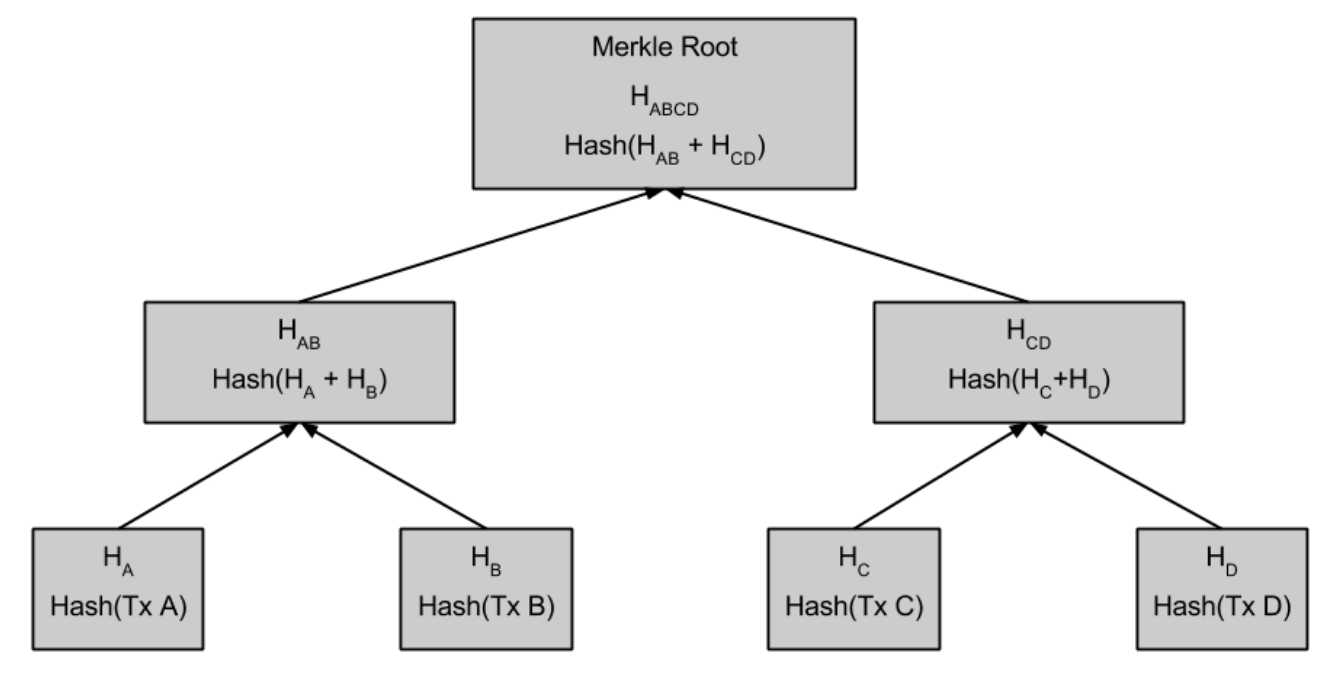
\includegraphics[width=0.6\columnwidth]{images/merkle.png}
  \end{center}
  \caption{Merkle Tree}
  \label{fig:merkle-tree}
\end{figure}

\section{Blockchain}

A blockchain is a decentralized, distributed, and oftentimes public, digital
ledger consisting of records called blocks that is used to record transactions
across many computers so that any involved block cannot be altered
retroactively, without the alteration of all subsequent blocks. This allows the
participants to verify and audit transactions independently and relatively
inexpensively. A blockchain database is managed autonomously using a
peer-to-peer network and a distributed timestamping server. They are
authenticated by mass collaboration powered by collective self-interests. Such
a design facilitates robust workflow where participants' uncertainty regarding
data security is marginal. The use of a blockchain removes the characteristic
of infinite reproducibility from a digital asset. It confirms that each unit of
value was transferred only once, solving the long-standing problem of double
spending. A blockchain has been described as a value-exchange protocol. A
blockchain can maintain title rights because, when properly set up to detail
the exchange agreement, it provides a record that compels offer and acceptance.

\subsection{Blocks}

Blocks hold batches of valid transactions that are hashed and encoded into a
Merkle tree. Each block includes the cryptographic hash of the prior block in
the blockchain, linking the two. The linked blocks form a chain. This iterative
process confirms the integrity of the previous block, all the way back to the
original genesis block. Sometimes separate blocks can be produced concurrently,
creating a temporary fork. In addition to a secure hash-based history, any
blockchain has a specified algorithm for scoring different versions of the
history so that one with a higher score can be selected over others. Blocks not
selected for inclusion in the chain are called orphan blocks. Peers supporting
the database have different versions of the history from time to time. They
keep only the highest-scoring version of the database known to them. Whenever a
peer receives a higher-scoring version (usually the old version with a single
new block added) they extend or overwrite their own database and retransmit the
improvement to their peers. There is never an absolute guarantee that any
particular entry will remain in the best version of the history forever.
Blockchains are typically built to add the score of new blocks onto old blocks
and are given incentives to extend with new blocks rather than overwrite old
blocks. Therefore, the probability of an entry becoming superseded decreases
exponentially as more blocks are built on top of it, eventually becoming very
low. For example, Bitcoin uses a proof-of-work system, where the chain with the
most cumulative proof-of-work is considered the valid one by the network. There
are a number of methods that can be used to demonstrate a sufficient level of
computation. Within a blockchain the computation is carried out redundantly
rather than in the traditional segregated and parallel manner.

\subsection{Block Time}

The block time is the average time it takes for the network to generate one
extra block in the blockchain. Some blockchains create a new block as
frequently as every five seconds. By the time of block completion, the included
data becomes verifiable. In cryptocurrency, this is practically when the
transaction takes place, so a shorter block time means faster transactions. The
block time for Ethereum is set to between 14 and 15 seconds, while for Bitcoin
it is on average 10 minutes.

\section{Bitcoin}

Bitcoin~\cite{nakamoto} is a cryptocurrency. It is a decentralized digital
currency without a central bank or single administrator that can be sent from
user to user on the peer-to-peer Bitcoin network without the need for
intermediaries.

Transactions are verified by network nodes through cryptography and recorded in
a public distributed ledger called a blockchain. Bitcoin was invented in 2008
by an unknown person or group of people using the name Satoshi Nakamoto and
started in 2009 when its source code was released as open-source software.
Bitcoins are created as a reward for a process known as mining. They can be
exchanged for other currencies, products, and services.

The Bitcoin blockchain is displayed in Figure~\ref{fig:Bitcoin-blockchain}.

\begin{figure}[H]
  \begin{center}
    \includegraphics[width=0.6\columnwidth]{images/Bitcoin-blockchain.png}
  \end{center}
  \caption{The Bitcoin blockchain}
  \label{fig:Bitcoin-blockchain}
\end{figure}

\subsection{Transactions}

Transactions are defined using a
Forth-like\footnote{\url{https://www.taygeta.com/forth/dpans.html}} scripting
language. Transactions consist of one or more inputs and one or more outputs.
When a user sends Bitcoins, the user designates each address and the amount of
Bitcoin being sent to that address in an output. To prevent double spending,
each input must refer to a previous unspent output in the blockchain. The use
of multiple inputs corresponds to the use of multiple coins in a cash
transaction. Since transactions can have multiple outputs, users can send
Bitcoins to multiple recipients in one transaction. As in a cash transaction,
the sum of inputs (coins used to pay) can exceed the intended sum of payments.
In such a case, an additional output is used, returning the change back to the
payer. Any input satoshis not accounted for in the transaction outputs become
the transaction fee.

\begin{figure}[H]
  \begin{center}
    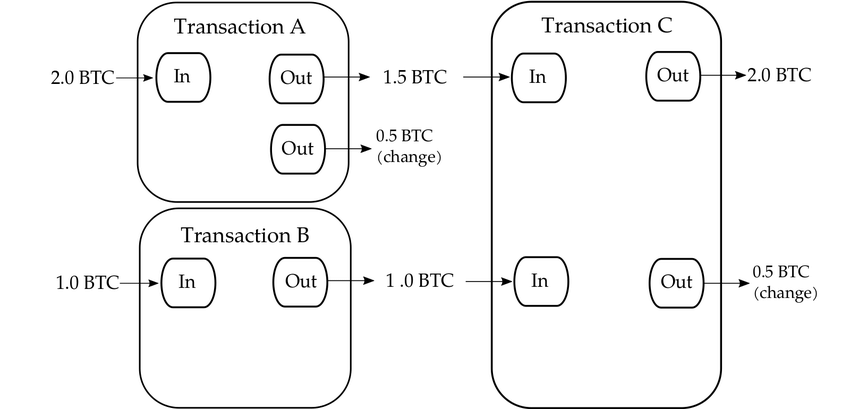
\includegraphics[width=0.6\columnwidth]{images/transactions.png}
  \end{center}
  \caption{Bitcoin transactions}
  \label{fig:transactions}
\end{figure}

\subsection{Mining}

Early Bitcoin miners used GPUs for mining, as they were better suited to the
proof-of-work algorithm than CPUs. Later amateurs mined Bitcoins with
specialized FPGA and ASIC chips. The chips pictured have become obsolete due to
increasing difficulty. Today, Bitcoin mining companies dedicate facilities to
housing and operating large amounts of high-performance mining hardware.
Semi-log plot of relative mining difficulty

Mining is a record-keeping service done through the use of computer processing
power. Miners keep the blockchain consistent, complete, and unalterable by
repeatedly grouping newly broadcast transactions into a block, which is then
broadcast to the network and verified by recipient nodes. Each block
contains a SHA-256 cryptographic hash of the previous block, thus linking
it to the previous block and giving the blockchain its name.

To be accepted by the rest of the network, a new block must contain a
proof-of-work (PoW). The system used is based on Adam Back's 1997 anti-spam
scheme, Hashcash~\cite{hashcash}. The PoW requires miners to find a
number called a nonce, such that when the block content is hashed along with
the nonce, the result is numerically smaller than the network's difficulty
target. This proof is easy for any node in the network to verify, but
extremely time-consuming to generate, as for a secure cryptographic hash,
miners must try many different nonce values (usually the sequence of tested
values is the ascending natural numbers: 0, 1, 2, 3, ... , 8) before
meeting the difficulty target.

Every 2,016 blocks (approximately 14 days at roughly 10 min per block), the
difficulty target is adjusted based on the network's recent performance, with
the aim of keeping the average time between new blocks at ten minutes. In this
way the system automatically adapts to the total amount of mining power on the
network. Between 1 March 2014 and 1 March 2015, the average number of
nonces miners had to try before creating a new block increased from 16.4
quintillion to 200.5 quintillion.

The proof-of-work system, alongside the chaining of blocks, makes modifications
of the blockchain extremely hard, as an attacker must modify all subsequent
blocks in order for the modifications of one block to be accepted. As new
blocks are mined all the time, the difficulty of modifying a block increases as
time passes and the number of subsequent blocks (also called confirmations of
the given block) increases.

\subsection{Simple payment verification - SPV}

The Bitcoin blockchain has generated more than 600,000 blocks since its
genesis\footnote{Genesis block is the first block mined in the blockchain}
block. At the time of writing, a full node needs about 250GB of disk space to
store the whole blockchain. Suppose a Bitcoin user wants to verify that their
transaction has been mined successfully to the main chain. The only way to do
it is to check the history of the transactions since the genesis block. Of
course, the user only cares about their transactions and not every transaction
that has ever occurred in the blockchain.

Satoshi's paper describes a method called the \textit {Simple payment
verification}(SPV) which tackles the problem in an efficient manner. Instead of
downloading the whole blockchain, the user can request from a full node only
the block headers. The size of all of the block headers of the main chain to
date is around 80MB which is easily manageable for modern computers and smart
phones. In order to avoid connecting to malicious nodes, it is often
recommended for users to connect to multiple nodes and request information
until they are convinced they have the longest chain. The longest chain is the
chain with the most proof of work and not the chain with the most blocks. To
prove that the network has accepted the transaction, the user has to link the
transaction to a certain block in the main chain and ensure that blocks are
added to the chain which means that more work is added to the chain.

\section{Ethereum}

Ethereum is an open source, public, blockchain-based distributed computing
platform featuring smart contract (scripting) functionality. Ether is the
cryptocurrency generated by the Ethereum platform as a reward to mining nodes
for computations performed and is the only currency accepted in the payment of
transaction fees on the platform. Ethereum is the second-largest
cryptocurrency platform by market capitalization, behind Bitcoin.

Ethereum provides a decentralized virtual machine, the Ethereum Virtual Machine
(EVM), which can execute scripts using an international network of public
nodes. The virtual machine's instruction set, in contrast to others like
Bitcoin Script, is Turing-complete. ``Gas'', an internal transaction pricing
mechanism, is used to mitigate spam and allocate resources on the network.

Ethereum was proposed in late 2013 by Vitalik Buterin, a cryptocurrency
researcher and programmer. Development was funded by an online crowdsale that
took place between July and August 2014. The system then went live on 30
July 2015, with 72 million coins minted. This accounts for about 65
percent of the total circulating supply in April 2020.

\subsection{Ethereum Virtual Machine}

The Ethereum Virtual Machine (EVM) is the runtime environment for smart
contracts in Ethereum. It is a 256-bit register stack, designed to run the same
code exactly as intended. It is the fundamental consensus mechanism for
Ethereum. The formal definition of the EVM is specified in the Ethereum Yellow
Paper. Ethereum Virtual Machines have been implemented in C++, C\#, Go,
Haskell, Java, JavaScript, Python, Ruby, Rust, Elixir, Erlang.

\subsection{Smart Contracts}

Ethereum's smart contracts are based on different computer languages, which
developers use to program their own functionalities. Smart contracts are
high-level programming abstractions that are compiled down to EVM bytecode and
deployed to the Ethereum blockchain for execution. They can be written in
Solidity (a language library with similarities to C and JavaScript), Serpent
(similar to Python, but deprecated), LLL (a low-level Lisp-like language), and
Mutan (Go-based, but deprecated). There is also a research-oriented language
under development called Vyper (a strongly-typed Python-derived decidable
language).

One issue related to using smart contracts on a public blockchain is that bugs,
including security holes, are visible to all but cannot be fixed quickly.
One example of this is the 17 June 2016 attack on The DAO, which could not be
quickly stopped or reversed.

There is ongoing research on how to use formal verification to express and
prove non-trivial properties. A Microsoft Research report noted that writing
solid smart contracts can be extremely difficult in practice, using The DAO
hack to illustrate this problem. The report discussed tools that Microsoft had
developed for verifying contracts, and noted that a large-scale analysis of
published contracts is likely to uncover widespread vulnerabilities. The report
also stated that it is possible to verify the equivalence of a Solidity program
and the EVM code.

\subsection{EVM Implementations}

\textbf{Py-EVM} is an evolving EVM which is created mainly for testing. The
ease of access and use, the configuration freedom of its underlying test chain
and its effectiveness for small size of data helped our first steps. However,
as the input data size started to grow, the effectiveness of the tool rapidly
fell.

\noindent
\textbf{Ganache} is a popular EVM developed by the Truffle team. Its
speed and configuration freedom are its main advantages. However, its extreme
memory requirement made it impossible to use when the sizes of the input became
analogous to the Bitcoin blockchain size.

\noindent
\textbf{Geth} is another popular EVM which is created by the Ethereum
team. It supports heavy customization while its memory usage is very limited
compared to Ganache, even for extensive inputs. It has, however, higher
execution times than Ganache for our purposes because Geth doesn't natively
support auto-mining. That is the capability to mine new blocks only when new
transactions are available. In order to avoid intense use of the CPU, we
injected a function in Geth's \texttt{miner} object be only invoked when a new
transaction is available. This, together with the fact that mining is
probabilistic, put an extra overhead at the execution time.

\section{Gas Profiling}

One useful utility we used is
solidity-gas-profiler\footnote{\url{https://github.com/yushih/solidity-gas-profiler}},
a profiling utility. This experimental software displays the gas usage in a
smart contract for each line of code. It gave us great insights regarding the
gas usage across contract’s functions, and consequently helped us target the
functionalities that needed to be refined. An example of the execution of the
gas profiled is displayed in listing~\ref{listing:gas-profile}

\lstinputlisting[language=Solidity, label={listing:gas-profile},
caption={Gas profile}]{code/GasProfile.sol}

\section{Non-Interactive Proofs Of Proof Of Work}

\subsection{Participants}

We consider a setting where the blockchain network consists of two different
types of nodes: The first kind, \emph{full nodes}, are responsible for the
maintenance of the chain including verifying it and mining new blocks. The
second kind, \emph{verifiers}, connect to full nodes and wish to learn facts
about the blockchain without downloading it, for example whether a particular
transaction is confirmed. The full nodes therefore also function as
\emph{provers} for the verifiers. Each verifier connects to multiple provers, at
least one of which is assumed to be honest.

\subsection{Blockchain Model} Each honest full node locally maintains a \emph{chain}
$\chain$, a sequence of blocks. In understanding that we are developing an
improvement on top of SPV, we use the term \emph{block} to mean what is
typically referred to as a \emph{block header}. Each block contains the Merkle
Tree root~\cite{merkle} of transaction data $\overline{x}$, the hash $s$ of the
previous block in the chain known as the \emph{previd}, as well as a nonce
value $ctr$. As discussed in the Introduction, the compression of application
data $\overline{x}$ is orthogonal to our goals in this paper and has been
explored in independent work~\cite{edrax} which can be composed with ours. Each
block $b = s \conc \overline{x} \conc ctr$ must satisfy the
proof-of-work~\cite{pow} equation $H(b) \leq T$ where $T$ is a constant
\emph{target}, a small value signifying the difficulty of the proof-of-work
problem. Our treatment is in the \emph{static difficulty} case, so we assume
that $T$ is constant throughout the execution\footnote{A treatment of variable
    difficulty NIPoPoWs has been explored in the soft fork
    case~\cite{dionyziz}, but we leave the treatment of velvet fork NIPoPoWs in
    the variable difficulty model for future work.}. $H(B)$ is known as the
    \emph{block id}.

Blockchains are finite block sequences obeying the \emph{blockchain property}:
that in every block in the chain there exists a pointer to its previous block. A
chain is \emph{anchored} if its first block is \emph{genesis}, denoted $\mathcal{G}$,
a special block known to all parties. This is the only block the verifier knows about
when it boots up. For chain addressing we use Python brackets $\chain[\cdot]$. A
zero-based positive number in a bracket indicates the indexed block in the
chain. A negative index indicates a block from the end, e.g., $\chain[-1]$ is
the tip of the blockchain. A range $\chain[i{:}j]$ is a subarray starting from
$i$ (inclusive) to j (exclusive). Given chains $\chain_1, \chain_2$ and blocks
$A, Z$ we concatenate them as $\chain_1 \chain_2$ or $\chain_1 A$ (if clarity
mandates it, we also use the symbol $\conc$ for concatenation). Here,
$\chain_2[0]$ must point to $\chain_1[-1]$ and $A$ must point to $\chain_1[-1]$.
We denote $\chain\{A{:}Z\}$ the subarray of the chain from block $A$ (inclusive) to
block $Z$ (exclusive). We can omit blocks or indices from either side of the range to
take the chain to the beginning or end respectively. As long as the blockchain
property is maintained, we freely use the set operators $\cup$, $\cap$ and
$\subseteq$ to denote operations between chains, implying that the appropriate
blocks are selected and then placed in chronological order.

During every round, every party attempts to \emph{mine} a new block on top of
its currently adopted chain. Each party is given $q$ queries to the random
oracle which it uses in attempting to mine a new block. Therefore the adversary
has $tq$ queries per round while the honest parties have $(n - t)q$ queries per
round. When an honest party discovers a new block, they extend their chain with
it and broadcast the new chain. Upon receiving a new chain $\chain'$ from the
network, an honest party compares its length $|\chain'|$ against its currently
adopted chain $\chain$ and adopts the newly received chain if it is longer. It
is assumed that the honest parties control the majority of the computational
power of the network. If so, the protocol
ensures consensus among the honest parties: There is a constant $k$, the
\emph{Common Prefix} parameter, such that, at any round, all the chains
belonging to honest parties share a common prefix of blocks; the chains can
deviate only up to $k$ blocks at the end of each chain~\cite{backbone}.
Concretely, if at some round $r$ two honest parties have $\chain_1$ and
$\chain_2$ respectively, then either $\chain_1[{:}-k]$ is a prefix of $\chain_2$
or $\chain_2[{:}-k]$ is a prefix of $\chain_1$.

\subsection{Superblocks}
Some valid blocks satisfy the proof-of-work equation better than required. If
a block $b$ satisfies $H(b) \leq 2^{-\mu} T$ for some natural number
$\mu \in \mathbb{N}$ we say that $b$ is a \emph{$\mu$-superblock} or a block
\emph{of level} $\mu$. The probability of a new valid block achieving level
$\mu$ is $2^{-\mu}$. The number of levels in the chain will be $\log|\chain|$
with high probability~\cite{popow}. Given a chain $\chain$, we denote
$\chain\upchain^\mu$ the subset of $\mu$-superblocks of $\chain$.

Non-Interactive Proofs of Proof-of-Work (NIPoPoW) protocols allow verifiers to
learn the most recent $k$ blocks of the blockchain adopted by an honest full
node without downloading the whole chain. The challenge lies in building a
verifier who can find the suffix of the longest chain between claims of both
honest and adversarial provers, while not downloading all block headers. Towards
that goal, the \emph{superblock} approach uses superblocks as samples of
proof-of-work. The prover sends superblocks to the verifier to convince them
that proof-of-work has taken place without actually presenting all this
proof-of-work. The protocol is parametrized by a constant security parameter
$m$. The parameter determines how many superblocks will be sent by the prover to
the verifier and security is proven with overwhelming probability in $m$.

\subsection{Prover} The prover is a friendly but untrusted node that
submits proofs of events that happen on a \emph{source} chain. These proofs are
advertised to a different \emph{target} chain and their validity is ensured by
other honest nodes. Provers need to monitor both source and target chains in
order to (a) create proofs of events from the source chain and (b) validate
proofs that are submitted by other nodes to the target chain.

The prover selects various levels $\mu$ and, for each
such level, sends a carefully chosen portion of its $\mu$-level
\emph{superchain} $\chain\upchain^\mu$ to the verifier. In standard blockchain
protocols such as Bitcoin and Ethereum, each block $\chain[i + 1]$ in $\chain$
points to its previous block $\chain[i]$, but each $\mu$-superblock
$\chain\upchain^\mu[i + 1]$ does not point to its previous $\mu$-superblock
$\chain\upchain^\mu[i]$. It is imperative that an adversarial prover does not
reorder the blocks within a superchain, but the verifier cannot verify this
unless each $\mu$-superblock points to its most recently preceding
$\mu$-superblock. The proposal is therefore to \emph{interlink} the chain by
having each $\mu$-superblock include an extra pointer to its most recently
preceding $\mu$-superblock. To ensure integrity, this pointer must be included
in the block header and verified by proof-of-work. However, the miner does not
know which level a candidate block will attain prior to mining it. For this
purpose, each block is proposed to include a pointer to the most recently
preceding $\mu$-superblock, for every $\mu$.
as illustrated in Figure~\ref{fig.hierarchy}.
As these levels are only $\log|\chain|$, this only adds $\log|\chain|$ extra
pointers to each block header.

Albeit a proof can be structurally correct, an adversary prover can dispatch a
proof of an dishonest chain. This is addressed by establishing a contest
period, in which honest provers can submit honest proofs that invalidate
the originally submitted. The rational behind this is that the honest chain
encapsulates the most proof-of-work, and thus achieves better score among
other proofs that represent shorter, dishonest chains. To provide incentives for honest
nodes to contest fraud proofs, a collateral is included to the submission of
proofs which is paid to the party that achieves to present a better proofs than
the originally submitted. If no contest happen, the collateral is returned to
the original issuer.
\begin{algorithm}
    \caption{\label{alg.nipopow-prover}The \textsf{Prove} algorithm
    for the NIPoPoW protocol in a soft fork}
    \begin{algorithmic}[1]
        \Function{\sf Prove$_{m,k}$}{$\chain$}
            \Let{B}{\chain[0]}
            \Comment{Genesis}
            \For{$\mu = |\chain[-k-1].\mathsf{interlink}|$ down to $0$}
                \Let{\alpha}{\chain[:-k]\{B:\}\upchain^\mu}
                \Let{\pi}{\pi \cup \alpha}
                \If{$m < |\alpha|$}
                    \Let{B}{\alpha[-m]}
                \EndIf
            \EndFor
            \Let{\chi}{\chain[-k:]}
            \State\Return{$\pi\chi$}
        \EndFunction
    \vskip8pt
    \end{algorithmic}
\end{algorithm}


\begin{figure}[ht]
    \centering
    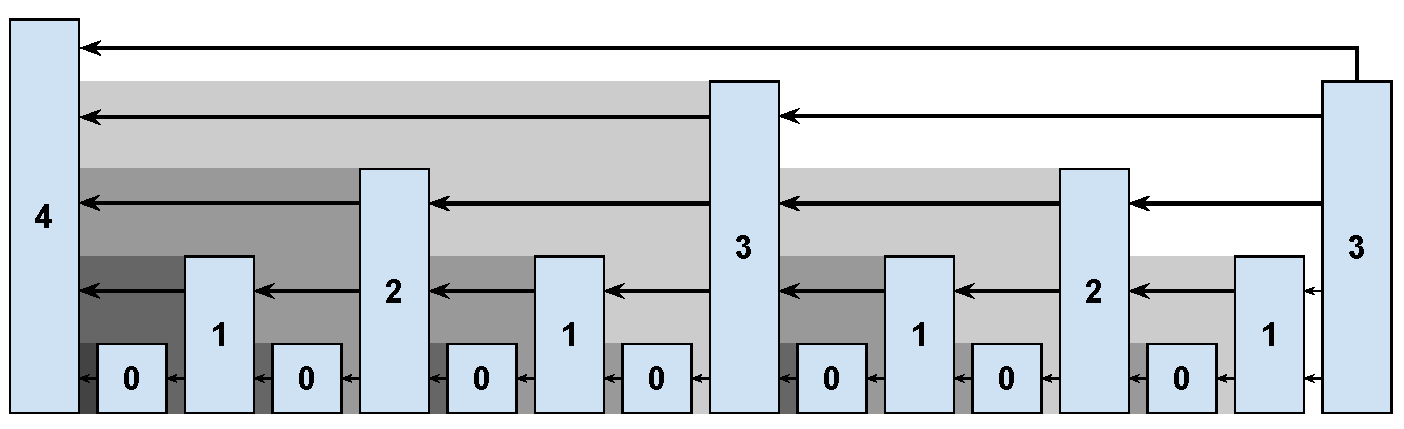
\includegraphics[width=0.9\columnwidth,keepaspectratio]{figures/prelims/level-shadows.pdf}
    \caption{The interlinked blockchain. Each superblock is drawn taller
    according to its achieved level. Each block links to all the blocks that are
    not being overshadowed by their descendants. The most recent (right-most)
    block links to the four blocks it has direct line-of-sight to.}
    \label{fig.hierarchy}
\end{figure}

\subsection{Verifier} The verifier is an application that performs
operations on proofs and does not need to be aware of the state of each chain.
Upon receiving two proofs, $\pi_1$ and $\pi_2$, the NIPoPoW verifier first
checks that they form valid chains. To check that they are valid chains, the
verifier ensures every block in the proof contains a pointer to its previous
block inside the proof through either the \emph{previd} pointer in the block
header, or in the interlink vector. If any of these checks fail, the proof is
rejected.  It then compares $\pi_1$ against $\pi_2$ using the $\leq_m$
operator, which works as follows. It finds the lowest common ancestor block $b
= (\pi_1 \cap \pi_2)[-1]$; that is, $b$ is the most recent block shared among
the two proofs.  Subsequently, it chooses the level $\mu_1$ for $\pi_1$ such
that $\lvert \pi_1\{b{:}\}\upchain^{\mu_1} \rvert \geq m$ (i.e., $\pi_1$ has at
least $m$ superblocks of level $\mu_1$ following block $b$) and the value
$2^{\mu_1} \lvert \pi_1\{b{:}\}\upchain^{\mu_1} \rvert$ is maximized.  It
chooses a level $\mu_2$ for $\pi_2$ in the same fashion. The two proofs are
compared by checking whether $2^{\mu_1} \lvert \pi_1\{b{:}\}\upchain^{\mu_1}
\rvert \geq 2^{\mu_2} \lvert \pi_2\{b{:}\}\upchain^{\mu_2} \rvert$ and the
proof with the largest score is deemed the winner. The comparison is
illustrated in Algorithm~\ref{alg.nipopow-verifier}.

\begin{algorithm}[H]
    \caption{\label{alg.nipopow-verifier}The \textsf{Verify} algorithm
    for the NIPoPoW protocol}
    \begin{algorithmic}[1]
        \Function{{\sf best-arg}$_m$}{$\pi, b$}
            \Let{M}{\{\mu: |\pi\upchain^\mu\{b:\}| \geq m\} \cup \{0\}}
            \Comment{Valid levels}
            \State\Return{$\max_{\mu \in M}\{2^\mu  \cdot |\pi\upchain^\mu\{b:\}|\}$}
            \Comment{Score for level}
        \EndFunction
        \Operator{$\pi_A \geq_m \pi_B$}
            \Let{b}{(\pi_A \cap \pi_B)[-1]}
              \Comment LCA
            \State\Return{$\textsf{best-arg}_m(\pi_A, b) \geq
                           \textsf{best-arg}_m(\pi_B, b)$}
        \EndOperator
        \Function{\sf Verify$^Q_{m,k}$}{$\mathcal{P}$}
            \Let{\tilde\pi}{(\text{Gen})}
              \Comment{Trivial anchored blockchain}
            \For{$(\pi, \chi) \in \mathcal{P}$}
                \Comment{Examine each proof in $\mathcal{P}$}
                \If{$\mathsf{validChain}(\pi \chi)
                    \land |\chi| = k
                    \land \pi \geq_m \tilde\pi$}
                    \State{$\tilde\pi \gets \pi$}
                    \State{$\tilde\chi \gets \chi$}
                    \Comment{Update current best}
                \EndIf
            \EndFor
            \State\Return{$\tilde{Q}(\tilde\chi)$}
        \EndFunction
    \vskip8pt
    \end{algorithmic}
\end{algorithm}


\begin{algorithm}
    \caption{\label{alg.nipopow-verifier-infix}The \textsf{verify} algorithm
    for the NIPoPoW infix protocol}
    \begin{algorithmic}[1]
        \Function{\sf ancestors}{$B, \textsf{blockById}$}
            \If{$B = \text{Gen}$}
                \State\Return{$\{B\}$}
            \EndIf
            \Let{\chain}{\emptyset}
            \For{$\textsf{id} \in B.\textsf{interlink}$}
                \If{$\textsf{id} \in \textsf{blockById}$}
                    \Let{B'}{\textsf{blockById}[\textsf{id}]}
                    \Comment{Collect into DAG}
                    \Let{\chain}{\chain \cup \textsf{ancestors}(B', \textsf{blockById})}
                \EndIf
            \EndFor
            \State\Return{$\chain \cup \{B\}$}
        \EndFunction
        \Function{\sf verify-infx$^D_{\ell,m,k}$}{$\mathcal{P}$}
            \Let{\textsf{blockById}}{\emptyset}
            \For{$(\pi, \chi) \in \mathcal{P}$}
                \For{$B \in \pi$}
                    \Let{\textsf{blockById}[\textsf{id}(B)]}{B}
                \EndFor
            \EndFor
            \Let{\tilde\pi}{\text{best }\pi\in\mathcal{P}\text{ according to suffix verifier}}
            \State\Return{$D(\textsf{ancestors}(\tilde\pi[-1],
            \textsf{blockById}))$}
        \EndFunction
    \vskip8pt
    \end{algorithmic}
\end{algorithm}


An adversary prover could skip the blocks of interest and present an honest and
longer chain that is considered a better proof. For that reason, the last step
of the algorithm in the suffix verifier is changed to not only store the best
proof but also combine the two proofs by including all of the ancestor blocks
of the losing proof. This is called infix verification and is guaranteed to
include the blocks of interest. The resulting best proof is stored as a
DAG(Directed Acyclic Graph), as in Algorithm~\ref{alg.nipopow-verifier-infix}.

The exact NIPoPoW protocol works like this: The prover holds a full chain
$\chain$. When the verifier requests a proof, the prover sends the last $k$
blocks of their chain, the suffix $\chi = \chain[-k{:}]$, in full. From the
larger prefix $\chain[{:}-k]$, the prover constructs a proof $\pi$ by selecting
certain superblocks as representative samples of the proof-of-work that took
place. The blocks are picked as follows. The prover selects the \emph{highest}
level $\mu^*$ that has at least $m$ blocks in it and includes all these blocks
in their proof (if no such level exists, the chain is small and can be sent in
full). The prover then iterates from level $\mu = \mu^* - 1$ down to $0$. For
every level $\mu$, it includes sufficient $\mu$-superblocks to cover the last
$m$ blocks of level $\mu + 1$, as illustrated in
Algorithm~\ref{alg.nipopow-prover}. Because the density of blocks doubles as
levels are descended, the proof will contain in expectation $2m$ blocks for each
level below $\mu^*$. As such, the total proof size $\pi \chi$ will be
$\Theta(m\log|\chain| + k)$. Such proofs that are polylogarithmic in the chain
size constitute an exponential improvement over traditional SPV clients and are
called \emph{succinct}.

\section{NIPoPoW Verifier in Solidity}

\subsection{Methodology}

Christogloy et. al. has provided a Solidity implementation. We used this
implementation as a basis for our work. Since we adopted common primitives, we
used some of the tools the authors used for functionalities such as
constructing blockchains and proofs. For the purposes of our implementation, we
to enhance the functionality of the existing tools in some cases. We are
thankful to the writers for sharing their implementation. This greatly
facilitated our work.

In this subsection, we describe the model of Non-Interactive Proofs of Proof of
Work in the context of the verifier implementation in Solidity. This includes
the following:

\begin{enumerate}
  \item
    Construction of a blockchain.
  \item
    Construction of a proof for an event in the blockchain.
  \item
    Verification of the proof.
\end{enumerate}

\subsubsection{Blockchain}

The tool that creates the blockchain has been created by Andrew Miller, one of
the writers of Non-Interactive Proofs of Proof of Work paper. The tool is using
the Bitcoin library\footnote{\url{https://pypi.org/project/bitcoinlib/}} to construct
a blockchain similar to Bitcoin’s. The interlink pointers are organized into a
Merkle Tree and the index is determined by their level. The Merkle root of the
interlink tree is a 32-bit value, and is included in the block header as an
additional value. The new size of the block header is 112 bytes. In order to
ensure security, it is important for the interlink root to be included in the
block header, as it is part of the proof. Otherwise, attackers could attack
the proofs by reordering or including stray blocks. Miners can easily verify
that the Merkle root is correct.

\subsubsection{Superblock Levels}

We assume that the difficulty target of mined blocks is constant. This is not
the actual setting of the Bitcoin blockchain. The definition of superblocks is
changed to a simpler definition and the level is determined by the number of
leading zeros of the block header hash. Although this change does not take into
account the difficulty target, the scoring of proofs does not generate security
holes in the protocol.

\subsubsection{Proof}

The tool for the creation of proofs has also been created by Andrew Miller. The
prover receives the following inputs:

\begin{itemize}
  \item
    A blockchain with interlinks
  \item
    The security parameter $k$
  \item
    The security parameter $m$
\end{itemize}

\subsection{Phases}

The goal of the verifier is to securely determine if an event has occurred in
the honest blockchain by examining proofs. A proof is submitted in combination
with a predicate. The proof is considered valid if it is constructively correct
and the predicate is evaluated against the submitted proof. The predicate
represents the existence of an event in the source blockchain, such as the
occurrence of a transaction. In this context, the predicate indicates the
existence of a block within the proof.

The verifier functions in two main phases: (a) \textbf{submit phase} and (b)
\textbf{contest phase}. Each phase has different input and functionality, and
is performed by different entities.

\subsubsection{Submit phase:} In \textbf{submit phase}, an entity submits a
proof and an event. We assume that at least one honest full node is aware of
the submission. This is also a part of the model of NIPoPoWs, and is a logical
assumption as explained in the NIPoPoW paper. In order to claim the occurrence
of an event, one must provide a proof and a predicate regarding the underlying
event.  If $r$ rounds pass, the value of the predicate becomes immutable. The
passing of rounds is indicated by the mining of new blocks atop of the block
containing the submitted proof. The value of the predicate can change if a
different prover successfully contests the submitted proof at some round $r_{c}
< r$.

\subsubsection{Contesting phase:} In \textbf{contesting phase}, a new proof is
submitted. If this proof has a better score, then the predicate is evaluated
against the new proof. The contesting proof is considered better only if it is
structurally correct and it represents a chain that encapsulates more proof-of-
work than the originally submitted proof, as described in the NIPoPoWs paper.
In order to contest, one must provide the new proof and the predicate that is
claimed to be \true by the originally submitted proof.\\

The functionality of a NIPoPoW verifier is the following:
\begin{itemize}

  \item
    If an \textit{honest} party submits a proof and no contest occurs, then
    the $predicate$ becomes $true$.

  \item
    If an \textit{honest} party submits a proof and it is contested by an
    \textit{adversary}, then the contest is unsuccessful and the
    $predicate$ remains $true$.

  \item
      If an \textit{adversary} submits a proof, then an \textit{honest} prover
      makes a contest. The contest invalidates the original submission and the
      $predicate$ becomes $false$.

  \item
    The scenario in which an \textit{adversary} submits a proof an
    \textit{honest} does not contest does not take place due to the
    assumption that at least one honest party observes the traffic of the
    contract.

\end{itemize}

\subsection{Considerations}

In order to construct a verifier, a Directed Acyclic Graph (DAG) is maintained
in storage. This structure is stored in the form of a hashmap, and is used
to host blocks of all different proofs. This process aims to prevent
adversarial proofs which are structurally valid but blocks are intentionally
skipped. Such a scenario is displayed in Figure~\ref{figure:DAG_usage}. The DAG
is then used to construct the ancestors structure by performing a simple graph
search. By iterating ancestors, we can securely determine the value of the
predicate.

\begin{figure}[h!]
    \centering
    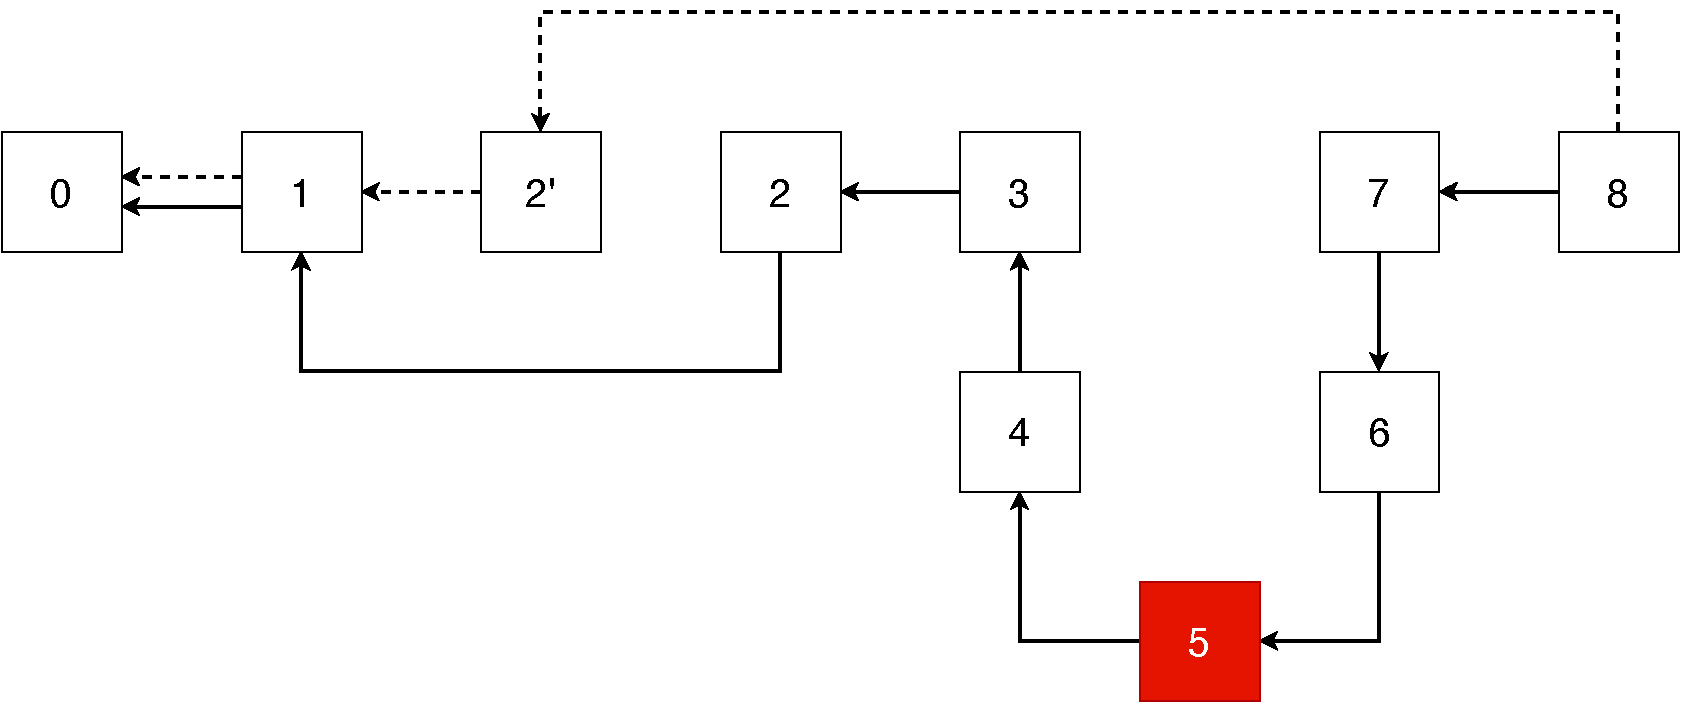
\includegraphics[width=8cm]{./images/DAG_usage.pdf}
    \caption{Combination of multiple proofs in a DAG. The red block is the
        block of interest. Honest proof consists of blocks connected by solid
        lines and adversarial proof by dashed lines. The adversary
        intentionally uses a different set of blocks.}
    \label{figure:DAG_usage}
\end{figure}


Reading from and writing to persistent memory are expensive operations in
Solidity~\cite{wood}. A summary of gas costs for storage and memory access if is
displayed in Table~\ref{table:ethereum_gas_list}. This fact was observed by
Giorgos et al.\ and was recognized as the bottleneck of the application.

\begin{table}[]
\centering
\begin{tabular}{@{}llr@{}}
\toprule
\multicolumn{1}{c}{Operation} & \multicolumn{1}{c}{Cost} & \multicolumn{1}{c}{Desc} \\
\midrule
$G_{create}$ & 32000 & Paid for a CREATE operation.\\
$G_{sload}$ & 200 & Paid for a SLOAD operation.\\
$G_{sset}$ & 20000 & Paid for an SSTORE operation.\\
$G_{memory}$ & 3 & Paid words expanding memory.\\
$G_{txdatazero}$ & 4 & Paid for zero byte of data for a transaction.\\
$G_{txdatanonzero}$ & 68 & Paid for non-zero byte of data for a transaction.\\
\end{tabular}
\caption{Ethereum gas list}
\label{table:ethereum_gas_list}
\end{table}


\subsubsection{Solidity Algorithm}

We describe each phase of the previous implementation in
Algorithm~\ref{alg:initial}.

\begin{algorithm}[H]

    \caption{\label{alg:initial}The \textsf{NIPoPoW} verifier implementation by
        Christoglou et.\ al.
    }
    \begin{algorithmic}[1]

    \Contract{crosschain}
    \State $\textsf{events} \gets \bot$
    \State $\textsf{DAG} \gets \bot$; $\textsf{ancestors} \gets \bot$
    \Function{\sf submit}{$\pis$, $e$}
        \State \textsf{require}($\textsf{events$[e]$} = \bot$)
        \State \textsf{require}($\textsf{valid-interlinks}(\pi)$)
        \State \textsf{events$[e].\pi$} $\gets$ $\pis$
        \State \textsf{DAG} $\gets$ \textsf{DAG} $\cup$ $\pi$
        \State \textsf{ancestors} $\gets$ \textsf{find-ancestors(DAG, $\pi$[-1])}
        \State \textsf{require}(\textsf{evaluate-predicate}(\textsf{ancestors}, e))
        \State \textsf{ancestors} $=$ $\bot$
        \EndFunction
    \Function{\sf contest}{$\pic$, $e$}
        \State \textsf{require}(\textsf{events}$[e]$ $\ne$ $\bot$)
        \State \textsf{require}(\textsf{valid-interlinks}($\pic$))
        \State $lca$ = \textsf{find-lca}($\textsf{events}[e].\pi$, $\pic$)
        \State \textsf{require}($\pic$ $\geq_m$ $\textsf{events}[e].\pi$)
        \State \textsf{DAG} $\gets$ \textsf{DAG} $\cup$ $\pic$
        \State \textsf{ancestors} $\gets$
        \textsf{find-ancestors}($\textsf{DAG}$, $\textsf{events}[e].\pi$[-1])
        \State \textsf{require}($\neg$\textsf{evaluate-predicate}(\textsf{ancestors}, $e$))
        \State \textsf{ancestors} $=$ $\bot$
        \State \textsf{events$[e]$} $\gets$ $\bot$
    \EndFunction
    \EndContract
    \vskip8pt
    \end{algorithmic}
\end{algorithm}


